% Created by tikzDevice version 0.12.6 on 2026-08-03 04:42:19
% !TEX encoding = UTF-8 Unicode
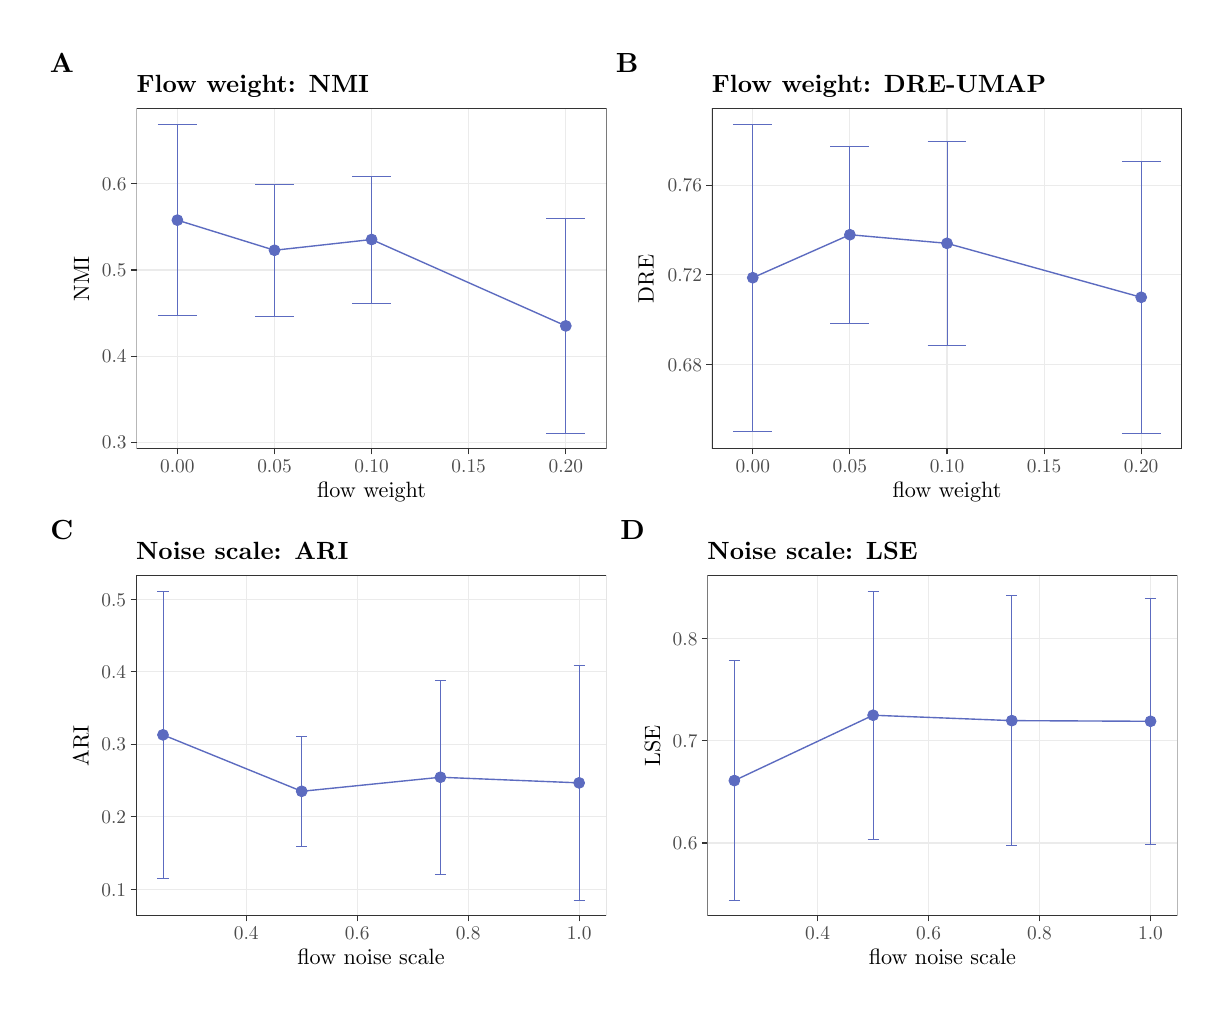
\begin{tikzpicture}[x=1pt,y=1pt]
\definecolor{fillColor}{RGB}{255,255,255}
\path[use as bounding box,fill=fillColor,fill opacity=0.00] (0,0) rectangle (423.43,348.50);
\begin{scope}
\path[clip] (  0.00,  0.00) rectangle (423.43,348.50);
\definecolor{drawColor}{RGB}{255,255,255}
\definecolor{fillColor}{RGB}{255,255,255}

\path[draw=drawColor,line width= 0.6pt,line join=round,line cap=round,fill=fillColor] (  0.00,  0.00) rectangle (423.43,348.50);
\end{scope}
\begin{scope}
\path[clip] (  5.50,174.25) rectangle (211.72,343.00);
\definecolor{drawColor}{RGB}{255,255,255}
\definecolor{fillColor}{RGB}{255,255,255}

\path[draw=drawColor,line width= 0.6pt,line join=round,line cap=round,fill=fillColor] (  5.50,174.25) rectangle (211.72,343.00);
\end{scope}
\begin{scope}
\path[clip] (211.72,174.25) rectangle (417.93,343.00);
\definecolor{drawColor}{RGB}{255,255,255}
\definecolor{fillColor}{RGB}{255,255,255}

\path[draw=drawColor,line width= 0.6pt,line join=round,line cap=round,fill=fillColor] (211.72,174.25) rectangle (417.93,343.00);
\end{scope}
\begin{scope}
\path[clip] (  6.02,174.81) rectangle (211.19,342.45);
\definecolor{drawColor}{RGB}{255,255,255}
\definecolor{fillColor}{RGB}{255,255,255}

\path[draw=drawColor,line width= 0.4pt,line join=round,line cap=round,fill=fillColor] (  6.02,174.81) rectangle (211.19,342.45);
\end{scope}
\begin{scope}
\path[clip] ( 39.36,196.28) rectangle (209.19,319.14);
\definecolor{fillColor}{RGB}{255,255,255}

\path[fill=fillColor] ( 39.36,196.28) rectangle (209.19,319.14);
\definecolor{drawColor}{gray}{0.92}

\path[draw=drawColor,line width= 0.4pt,line join=round] ( 39.36,198.69) --
	(209.19,198.69);

\path[draw=drawColor,line width= 0.4pt,line join=round] ( 39.36,229.80) --
	(209.19,229.80);

\path[draw=drawColor,line width= 0.4pt,line join=round] ( 39.36,260.92) --
	(209.19,260.92);

\path[draw=drawColor,line width= 0.4pt,line join=round] ( 39.36,292.03) --
	(209.19,292.03);

\path[draw=drawColor,line width= 0.4pt,line join=round] ( 54.10,196.28) --
	( 54.10,319.14);

\path[draw=drawColor,line width= 0.4pt,line join=round] ( 89.19,196.28) --
	( 89.19,319.14);

\path[draw=drawColor,line width= 0.4pt,line join=round] (124.28,196.28) --
	(124.28,319.14);

\path[draw=drawColor,line width= 0.4pt,line join=round] (159.36,196.28) --
	(159.36,319.14);

\path[draw=drawColor,line width= 0.4pt,line join=round] (194.45,196.28) --
	(194.45,319.14);
\definecolor{drawColor}{RGB}{92,107,192}

\path[draw=drawColor,line width= 0.5pt,line join=round] ( 54.10,278.95) --
	( 89.19,268.06) --
	(124.28,271.95) --
	(194.45,240.73);
\definecolor{fillColor}{RGB}{92,107,192}

\path[draw=drawColor,line width= 0.3pt,line join=round,line cap=round,fill=fillColor] ( 54.10,278.95) circle (  1.97);

\path[draw=drawColor,line width= 0.3pt,line join=round,line cap=round,fill=fillColor] ( 89.19,268.06) circle (  1.97);

\path[draw=drawColor,line width= 0.3pt,line join=round,line cap=round,fill=fillColor] (124.28,271.95) circle (  1.97);

\path[draw=drawColor,line width= 0.3pt,line join=round,line cap=round,fill=fillColor] (194.45,240.73) circle (  1.97);

\path[draw=drawColor,line width= 0.3pt,line join=round] ( 47.08,313.55) --
	( 61.11,313.55);

\path[draw=drawColor,line width= 0.3pt,line join=round] ( 54.10,313.55) --
	( 54.10,244.35);

\path[draw=drawColor,line width= 0.3pt,line join=round] ( 47.08,244.35) --
	( 61.11,244.35);

\path[draw=drawColor,line width= 0.3pt,line join=round] ( 82.17,291.89) --
	( 96.20,291.89);

\path[draw=drawColor,line width= 0.3pt,line join=round] ( 89.19,291.89) --
	( 89.19,244.24);

\path[draw=drawColor,line width= 0.3pt,line join=round] ( 82.17,244.24) --
	( 96.20,244.24);

\path[draw=drawColor,line width= 0.3pt,line join=round] (117.26,294.88) --
	(131.29,294.88);

\path[draw=drawColor,line width= 0.3pt,line join=round] (124.28,294.88) --
	(124.28,249.02);

\path[draw=drawColor,line width= 0.3pt,line join=round] (117.26,249.02) --
	(131.29,249.02);

\path[draw=drawColor,line width= 0.3pt,line join=round] (187.44,279.60) --
	(201.47,279.60);

\path[draw=drawColor,line width= 0.3pt,line join=round] (194.45,279.60) --
	(194.45,201.86);

\path[draw=drawColor,line width= 0.3pt,line join=round] (187.44,201.86) --
	(201.47,201.86);
\definecolor{drawColor}{gray}{0.20}

\path[draw=drawColor,line width= 0.4pt,line join=round,line cap=round] ( 39.36,196.28) rectangle (209.19,319.14);
\end{scope}
\begin{scope}
\path[clip] (  0.00,  0.00) rectangle (423.43,348.50);
\definecolor{drawColor}{gray}{0.30}

\node[text=drawColor,anchor=base east,inner sep=0pt, outer sep=0pt, scale=  0.70] at ( 35.76,196.28) {0.3};

\node[text=drawColor,anchor=base east,inner sep=0pt, outer sep=0pt, scale=  0.70] at ( 35.76,227.39) {0.4};

\node[text=drawColor,anchor=base east,inner sep=0pt, outer sep=0pt, scale=  0.70] at ( 35.76,258.50) {0.5};

\node[text=drawColor,anchor=base east,inner sep=0pt, outer sep=0pt, scale=  0.70] at ( 35.76,289.62) {0.6};
\end{scope}
\begin{scope}
\path[clip] (  0.00,  0.00) rectangle (423.43,348.50);
\definecolor{drawColor}{gray}{0.20}

\path[draw=drawColor,line width= 0.4pt,line join=round] ( 37.36,198.69) --
	( 39.36,198.69);

\path[draw=drawColor,line width= 0.4pt,line join=round] ( 37.36,229.80) --
	( 39.36,229.80);

\path[draw=drawColor,line width= 0.4pt,line join=round] ( 37.36,260.92) --
	( 39.36,260.92);

\path[draw=drawColor,line width= 0.4pt,line join=round] ( 37.36,292.03) --
	( 39.36,292.03);
\end{scope}
\begin{scope}
\path[clip] (  0.00,  0.00) rectangle (423.43,348.50);
\definecolor{drawColor}{gray}{0.20}

\path[draw=drawColor,line width= 0.4pt,line join=round] ( 54.10,194.28) --
	( 54.10,196.28);

\path[draw=drawColor,line width= 0.4pt,line join=round] ( 89.19,194.28) --
	( 89.19,196.28);

\path[draw=drawColor,line width= 0.4pt,line join=round] (124.28,194.28) --
	(124.28,196.28);

\path[draw=drawColor,line width= 0.4pt,line join=round] (159.36,194.28) --
	(159.36,196.28);

\path[draw=drawColor,line width= 0.4pt,line join=round] (194.45,194.28) --
	(194.45,196.28);
\end{scope}
\begin{scope}
\path[clip] (  0.00,  0.00) rectangle (423.43,348.50);
\definecolor{drawColor}{gray}{0.30}

\node[text=drawColor,anchor=base,inner sep=0pt, outer sep=0pt, scale=  0.70] at ( 54.10,187.86) {0.00};

\node[text=drawColor,anchor=base,inner sep=0pt, outer sep=0pt, scale=  0.70] at ( 89.19,187.86) {0.05};

\node[text=drawColor,anchor=base,inner sep=0pt, outer sep=0pt, scale=  0.70] at (124.28,187.86) {0.10};

\node[text=drawColor,anchor=base,inner sep=0pt, outer sep=0pt, scale=  0.70] at (159.36,187.86) {0.15};

\node[text=drawColor,anchor=base,inner sep=0pt, outer sep=0pt, scale=  0.70] at (194.45,187.86) {0.20};
\end{scope}
\begin{scope}
\path[clip] (  0.00,  0.00) rectangle (423.43,348.50);
\definecolor{drawColor}{RGB}{0,0,0}

\node[text=drawColor,anchor=base,inner sep=0pt, outer sep=0pt, scale=  0.80] at (124.28,178.58) {flow weight};
\end{scope}
\begin{scope}
\path[clip] (  0.00,  0.00) rectangle (423.43,348.50);
\definecolor{drawColor}{RGB}{0,0,0}

\node[text=drawColor,rotate= 90.00,anchor=base,inner sep=0pt, outer sep=0pt, scale=  0.80] at ( 22.22,257.71) {NMI};
\end{scope}
\begin{scope}
\path[clip] (  0.00,  0.00) rectangle (423.43,348.50);
\definecolor{drawColor}{RGB}{0,0,0}

\node[text=drawColor,anchor=base west,inner sep=0pt, outer sep=0pt, scale=  0.90] at ( 39.36,325.12) {\bfseries Flow weight: NMI};
\end{scope}
\begin{scope}
\path[clip] (  0.00,  0.00) rectangle (423.43,348.50);
\definecolor{drawColor}{RGB}{0,0,0}

\node[text=drawColor,anchor=base,inner sep=0pt, outer sep=0pt, scale=  1.00] at ( 12.37,332.44) {\bfseries A};
\end{scope}
\begin{scope}
\path[clip] (210.54,174.81) rectangle (419.10,342.45);
\definecolor{drawColor}{RGB}{255,255,255}
\definecolor{fillColor}{RGB}{255,255,255}

\path[draw=drawColor,line width= 0.4pt,line join=round,line cap=round,fill=fillColor] (210.54,174.81) rectangle (419.10,342.45);
\end{scope}
\begin{scope}
\path[clip] (247.27,196.28) rectangle (417.10,319.14);
\definecolor{fillColor}{RGB}{255,255,255}

\path[fill=fillColor] (247.27,196.28) rectangle (417.10,319.14);
\definecolor{drawColor}{gray}{0.92}

\path[draw=drawColor,line width= 0.4pt,line join=round] (247.27,226.78) --
	(417.10,226.78);

\path[draw=drawColor,line width= 0.4pt,line join=round] (247.27,259.20) --
	(417.10,259.20);

\path[draw=drawColor,line width= 0.4pt,line join=round] (247.27,291.62) --
	(417.10,291.62);

\path[draw=drawColor,line width= 0.4pt,line join=round] (262.01,196.28) --
	(262.01,319.14);

\path[draw=drawColor,line width= 0.4pt,line join=round] (297.10,196.28) --
	(297.10,319.14);

\path[draw=drawColor,line width= 0.4pt,line join=round] (332.19,196.28) --
	(332.19,319.14);

\path[draw=drawColor,line width= 0.4pt,line join=round] (367.28,196.28) --
	(367.28,319.14);

\path[draw=drawColor,line width= 0.4pt,line join=round] (402.37,196.28) --
	(402.37,319.14);
\definecolor{drawColor}{RGB}{92,107,192}

\path[draw=drawColor,line width= 0.5pt,line join=round] (262.01,258.14) --
	(297.10,273.68) --
	(332.19,270.57) --
	(402.37,251.07);
\definecolor{fillColor}{RGB}{92,107,192}

\path[draw=drawColor,line width= 0.3pt,line join=round,line cap=round,fill=fillColor] (262.01,258.14) circle (  1.97);

\path[draw=drawColor,line width= 0.3pt,line join=round,line cap=round,fill=fillColor] (297.10,273.68) circle (  1.97);

\path[draw=drawColor,line width= 0.3pt,line join=round,line cap=round,fill=fillColor] (332.19,270.57) circle (  1.97);

\path[draw=drawColor,line width= 0.3pt,line join=round,line cap=round,fill=fillColor] (402.37,251.07) circle (  1.97);

\path[draw=drawColor,line width= 0.3pt,line join=round] (254.99,313.55) --
	(269.03,313.55);

\path[draw=drawColor,line width= 0.3pt,line join=round] (262.01,313.55) --
	(262.01,202.73);

\path[draw=drawColor,line width= 0.3pt,line join=round] (254.99,202.73) --
	(269.03,202.73);

\path[draw=drawColor,line width= 0.3pt,line join=round] (290.08,305.60) --
	(304.11,305.60);

\path[draw=drawColor,line width= 0.3pt,line join=round] (297.10,305.60) --
	(297.10,241.76);

\path[draw=drawColor,line width= 0.3pt,line join=round] (290.08,241.76) --
	(304.11,241.76);

\path[draw=drawColor,line width= 0.3pt,line join=round] (325.17,307.34) --
	(339.20,307.34);

\path[draw=drawColor,line width= 0.3pt,line join=round] (332.19,307.34) --
	(332.19,233.79);

\path[draw=drawColor,line width= 0.3pt,line join=round] (325.17,233.79) --
	(339.20,233.79);

\path[draw=drawColor,line width= 0.3pt,line join=round] (395.35,300.27) --
	(409.38,300.27);

\path[draw=drawColor,line width= 0.3pt,line join=round] (402.37,300.27) --
	(402.37,201.86);

\path[draw=drawColor,line width= 0.3pt,line join=round] (395.35,201.86) --
	(409.38,201.86);
\definecolor{drawColor}{gray}{0.20}

\path[draw=drawColor,line width= 0.4pt,line join=round,line cap=round] (247.27,196.28) rectangle (417.10,319.14);
\end{scope}
\begin{scope}
\path[clip] (  0.00,  0.00) rectangle (423.43,348.50);
\definecolor{drawColor}{gray}{0.30}

\node[text=drawColor,anchor=base east,inner sep=0pt, outer sep=0pt, scale=  0.70] at (243.67,224.37) {0.68};

\node[text=drawColor,anchor=base east,inner sep=0pt, outer sep=0pt, scale=  0.70] at (243.67,256.79) {0.72};

\node[text=drawColor,anchor=base east,inner sep=0pt, outer sep=0pt, scale=  0.70] at (243.67,289.21) {0.76};
\end{scope}
\begin{scope}
\path[clip] (  0.00,  0.00) rectangle (423.43,348.50);
\definecolor{drawColor}{gray}{0.20}

\path[draw=drawColor,line width= 0.4pt,line join=round] (245.27,226.78) --
	(247.27,226.78);

\path[draw=drawColor,line width= 0.4pt,line join=round] (245.27,259.20) --
	(247.27,259.20);

\path[draw=drawColor,line width= 0.4pt,line join=round] (245.27,291.62) --
	(247.27,291.62);
\end{scope}
\begin{scope}
\path[clip] (  0.00,  0.00) rectangle (423.43,348.50);
\definecolor{drawColor}{gray}{0.20}

\path[draw=drawColor,line width= 0.4pt,line join=round] (262.01,194.28) --
	(262.01,196.28);

\path[draw=drawColor,line width= 0.4pt,line join=round] (297.10,194.28) --
	(297.10,196.28);

\path[draw=drawColor,line width= 0.4pt,line join=round] (332.19,194.28) --
	(332.19,196.28);

\path[draw=drawColor,line width= 0.4pt,line join=round] (367.28,194.28) --
	(367.28,196.28);

\path[draw=drawColor,line width= 0.4pt,line join=round] (402.37,194.28) --
	(402.37,196.28);
\end{scope}
\begin{scope}
\path[clip] (  0.00,  0.00) rectangle (423.43,348.50);
\definecolor{drawColor}{gray}{0.30}

\node[text=drawColor,anchor=base,inner sep=0pt, outer sep=0pt, scale=  0.70] at (262.01,187.86) {0.00};

\node[text=drawColor,anchor=base,inner sep=0pt, outer sep=0pt, scale=  0.70] at (297.10,187.86) {0.05};

\node[text=drawColor,anchor=base,inner sep=0pt, outer sep=0pt, scale=  0.70] at (332.19,187.86) {0.10};

\node[text=drawColor,anchor=base,inner sep=0pt, outer sep=0pt, scale=  0.70] at (367.28,187.86) {0.15};

\node[text=drawColor,anchor=base,inner sep=0pt, outer sep=0pt, scale=  0.70] at (402.37,187.86) {0.20};
\end{scope}
\begin{scope}
\path[clip] (  0.00,  0.00) rectangle (423.43,348.50);
\definecolor{drawColor}{RGB}{0,0,0}

\node[text=drawColor,anchor=base,inner sep=0pt, outer sep=0pt, scale=  0.80] at (332.19,178.58) {flow weight};
\end{scope}
\begin{scope}
\path[clip] (  0.00,  0.00) rectangle (423.43,348.50);
\definecolor{drawColor}{RGB}{0,0,0}

\node[text=drawColor,rotate= 90.00,anchor=base,inner sep=0pt, outer sep=0pt, scale=  0.80] at (226.23,257.71) {DRE};
\end{scope}
\begin{scope}
\path[clip] (  0.00,  0.00) rectangle (423.43,348.50);
\definecolor{drawColor}{RGB}{0,0,0}

\node[text=drawColor,anchor=base west,inner sep=0pt, outer sep=0pt, scale=  0.90] at (247.27,325.12) {\bfseries Flow weight: DRE-UMAP};
\end{scope}
\begin{scope}
\path[clip] (  0.00,  0.00) rectangle (423.43,348.50);
\definecolor{drawColor}{RGB}{0,0,0}

\node[text=drawColor,anchor=base,inner sep=0pt, outer sep=0pt, scale=  1.00] at (216.63,332.44) {\bfseries B};
\end{scope}
\begin{scope}
\path[clip] (  5.50,  5.50) rectangle (211.72,174.25);
\definecolor{drawColor}{RGB}{255,255,255}
\definecolor{fillColor}{RGB}{255,255,255}

\path[draw=drawColor,line width= 0.6pt,line join=round,line cap=round,fill=fillColor] (  5.50,  5.50) rectangle (211.72,174.25);
\end{scope}
\begin{scope}
\path[clip] (211.72,  5.50) rectangle (417.93,174.25);
\definecolor{drawColor}{RGB}{255,255,255}
\definecolor{fillColor}{RGB}{255,255,255}

\path[draw=drawColor,line width= 0.6pt,line join=round,line cap=round,fill=fillColor] (211.72,  5.50) rectangle (417.93,174.25);
\end{scope}
\begin{scope}
\path[clip] (  6.22,  6.06) rectangle (211.00,173.69);
\definecolor{drawColor}{RGB}{255,255,255}
\definecolor{fillColor}{RGB}{255,255,255}

\path[draw=drawColor,line width= 0.4pt,line join=round,line cap=round,fill=fillColor] (  6.22,  6.06) rectangle (211.00,173.69);
\end{scope}
\begin{scope}
\path[clip] ( 39.16, 27.53) rectangle (209.00,150.39);
\definecolor{fillColor}{RGB}{255,255,255}

\path[fill=fillColor] ( 39.16, 27.53) rectangle (209.00,150.39);
\definecolor{drawColor}{gray}{0.92}

\path[draw=drawColor,line width= 0.4pt,line join=round] ( 39.16, 37.14) --
	(209.00, 37.14);

\path[draw=drawColor,line width= 0.4pt,line join=round] ( 39.16, 63.34) --
	(209.00, 63.34);

\path[draw=drawColor,line width= 0.4pt,line join=round] ( 39.16, 89.54) --
	(209.00, 89.54);

\path[draw=drawColor,line width= 0.4pt,line join=round] ( 39.16,115.73) --
	(209.00,115.73);

\path[draw=drawColor,line width= 0.4pt,line join=round] ( 39.16,141.93) --
	(209.00,141.93);

\path[draw=drawColor,line width= 0.4pt,line join=round] ( 78.97, 27.53) --
	( 78.97,150.39);

\path[draw=drawColor,line width= 0.4pt,line join=round] (119.07, 27.53) --
	(119.07,150.39);

\path[draw=drawColor,line width= 0.4pt,line join=round] (159.17, 27.53) --
	(159.17,150.39);

\path[draw=drawColor,line width= 0.4pt,line join=round] (199.27, 27.53) --
	(199.27,150.39);
\definecolor{drawColor}{RGB}{92,107,192}

\path[draw=drawColor,line width= 0.5pt,line join=round] ( 48.89, 92.96) --
	( 99.02, 72.56) --
	(149.14, 77.64) --
	(199.27, 75.61);
\definecolor{fillColor}{RGB}{92,107,192}

\path[draw=drawColor,line width= 0.3pt,line join=round,line cap=round,fill=fillColor] ( 48.89, 92.96) circle (  1.97);

\path[draw=drawColor,line width= 0.3pt,line join=round,line cap=round,fill=fillColor] ( 99.02, 72.56) circle (  1.97);

\path[draw=drawColor,line width= 0.3pt,line join=round,line cap=round,fill=fillColor] (149.14, 77.64) circle (  1.97);

\path[draw=drawColor,line width= 0.3pt,line join=round,line cap=round,fill=fillColor] (199.27, 75.61) circle (  1.97);

\path[draw=drawColor,line width= 0.3pt,line join=round] ( 46.88,144.80) --
	( 50.89,144.80);

\path[draw=drawColor,line width= 0.3pt,line join=round] ( 48.89,144.80) --
	( 48.89, 41.11);

\path[draw=drawColor,line width= 0.3pt,line join=round] ( 46.88, 41.11) --
	( 50.89, 41.11);

\path[draw=drawColor,line width= 0.3pt,line join=round] ( 97.01, 92.52) --
	(101.02, 92.52);

\path[draw=drawColor,line width= 0.3pt,line join=round] ( 99.02, 92.52) --
	( 99.02, 52.59);

\path[draw=drawColor,line width= 0.3pt,line join=round] ( 97.01, 52.59) --
	(101.02, 52.59);

\path[draw=drawColor,line width= 0.3pt,line join=round] (147.14,112.66) --
	(151.15,112.66);

\path[draw=drawColor,line width= 0.3pt,line join=round] (149.14,112.66) --
	(149.14, 42.62);

\path[draw=drawColor,line width= 0.3pt,line join=round] (147.14, 42.62) --
	(151.15, 42.62);

\path[draw=drawColor,line width= 0.3pt,line join=round] (197.27,118.11) --
	(201.28,118.11);

\path[draw=drawColor,line width= 0.3pt,line join=round] (199.27,118.11) --
	(199.27, 33.11);

\path[draw=drawColor,line width= 0.3pt,line join=round] (197.27, 33.11) --
	(201.28, 33.11);
\definecolor{drawColor}{gray}{0.20}

\path[draw=drawColor,line width= 0.4pt,line join=round,line cap=round] ( 39.16, 27.53) rectangle (209.00,150.39);
\end{scope}
\begin{scope}
\path[clip] (  0.00,  0.00) rectangle (423.43,348.50);
\definecolor{drawColor}{gray}{0.30}

\node[text=drawColor,anchor=base east,inner sep=0pt, outer sep=0pt, scale=  0.70] at ( 35.56, 34.73) {0.1};

\node[text=drawColor,anchor=base east,inner sep=0pt, outer sep=0pt, scale=  0.70] at ( 35.56, 60.93) {0.2};

\node[text=drawColor,anchor=base east,inner sep=0pt, outer sep=0pt, scale=  0.70] at ( 35.56, 87.13) {0.3};

\node[text=drawColor,anchor=base east,inner sep=0pt, outer sep=0pt, scale=  0.70] at ( 35.56,113.32) {0.4};

\node[text=drawColor,anchor=base east,inner sep=0pt, outer sep=0pt, scale=  0.70] at ( 35.56,139.52) {0.5};
\end{scope}
\begin{scope}
\path[clip] (  0.00,  0.00) rectangle (423.43,348.50);
\definecolor{drawColor}{gray}{0.20}

\path[draw=drawColor,line width= 0.4pt,line join=round] ( 37.16, 37.14) --
	( 39.16, 37.14);

\path[draw=drawColor,line width= 0.4pt,line join=round] ( 37.16, 63.34) --
	( 39.16, 63.34);

\path[draw=drawColor,line width= 0.4pt,line join=round] ( 37.16, 89.54) --
	( 39.16, 89.54);

\path[draw=drawColor,line width= 0.4pt,line join=round] ( 37.16,115.73) --
	( 39.16,115.73);

\path[draw=drawColor,line width= 0.4pt,line join=round] ( 37.16,141.93) --
	( 39.16,141.93);
\end{scope}
\begin{scope}
\path[clip] (  0.00,  0.00) rectangle (423.43,348.50);
\definecolor{drawColor}{gray}{0.20}

\path[draw=drawColor,line width= 0.4pt,line join=round] ( 78.97, 25.53) --
	( 78.97, 27.53);

\path[draw=drawColor,line width= 0.4pt,line join=round] (119.07, 25.53) --
	(119.07, 27.53);

\path[draw=drawColor,line width= 0.4pt,line join=round] (159.17, 25.53) --
	(159.17, 27.53);

\path[draw=drawColor,line width= 0.4pt,line join=round] (199.27, 25.53) --
	(199.27, 27.53);
\end{scope}
\begin{scope}
\path[clip] (  0.00,  0.00) rectangle (423.43,348.50);
\definecolor{drawColor}{gray}{0.30}

\node[text=drawColor,anchor=base,inner sep=0pt, outer sep=0pt, scale=  0.70] at ( 78.97, 19.11) {0.4};

\node[text=drawColor,anchor=base,inner sep=0pt, outer sep=0pt, scale=  0.70] at (119.07, 19.11) {0.6};

\node[text=drawColor,anchor=base,inner sep=0pt, outer sep=0pt, scale=  0.70] at (159.17, 19.11) {0.8};

\node[text=drawColor,anchor=base,inner sep=0pt, outer sep=0pt, scale=  0.70] at (199.27, 19.11) {1.0};
\end{scope}
\begin{scope}
\path[clip] (  0.00,  0.00) rectangle (423.43,348.50);
\definecolor{drawColor}{RGB}{0,0,0}

\node[text=drawColor,anchor=base,inner sep=0pt, outer sep=0pt, scale=  0.80] at (124.08,  9.83) {flow noise scale};
\end{scope}
\begin{scope}
\path[clip] (  0.00,  0.00) rectangle (423.43,348.50);
\definecolor{drawColor}{RGB}{0,0,0}

\node[text=drawColor,rotate= 90.00,anchor=base,inner sep=0pt, outer sep=0pt, scale=  0.80] at ( 22.03, 88.96) {ARI};
\end{scope}
\begin{scope}
\path[clip] (  0.00,  0.00) rectangle (423.43,348.50);
\definecolor{drawColor}{RGB}{0,0,0}

\node[text=drawColor,anchor=base west,inner sep=0pt, outer sep=0pt, scale=  0.90] at ( 39.16,156.37) {\bfseries Noise scale: ARI};
\end{scope}
\begin{scope}
\path[clip] (  0.00,  0.00) rectangle (423.43,348.50);
\definecolor{drawColor}{RGB}{0,0,0}

\node[text=drawColor,anchor=base,inner sep=0pt, outer sep=0pt, scale=  1.00] at ( 12.37,163.69) {\bfseries C};
\end{scope}
\begin{scope}
\path[clip] (212.18,  6.06) rectangle (417.47,173.69);
\definecolor{drawColor}{RGB}{255,255,255}
\definecolor{fillColor}{RGB}{255,255,255}

\path[draw=drawColor,line width= 0.4pt,line join=round,line cap=round,fill=fillColor] (212.18,  6.06) rectangle (417.47,173.69);
\end{scope}
\begin{scope}
\path[clip] (245.64, 27.53) rectangle (415.47,150.39);
\definecolor{fillColor}{RGB}{255,255,255}

\path[fill=fillColor] (245.64, 27.53) rectangle (415.47,150.39);
\definecolor{drawColor}{gray}{0.92}

\path[draw=drawColor,line width= 0.4pt,line join=round] (245.64, 53.88) --
	(415.47, 53.88);

\path[draw=drawColor,line width= 0.4pt,line join=round] (245.64, 90.82) --
	(415.47, 90.82);

\path[draw=drawColor,line width= 0.4pt,line join=round] (245.64,127.76) --
	(415.47,127.76);

\path[draw=drawColor,line width= 0.4pt,line join=round] (285.44, 27.53) --
	(285.44,150.39);

\path[draw=drawColor,line width= 0.4pt,line join=round] (325.54, 27.53) --
	(325.54,150.39);

\path[draw=drawColor,line width= 0.4pt,line join=round] (365.64, 27.53) --
	(365.64,150.39);

\path[draw=drawColor,line width= 0.4pt,line join=round] (405.75, 27.53) --
	(405.75,150.39);
\definecolor{drawColor}{RGB}{92,107,192}

\path[draw=drawColor,line width= 0.5pt,line join=round] (255.36, 76.44) --
	(305.49,100.05) --
	(355.62, 98.10) --
	(405.75, 97.86);
\definecolor{fillColor}{RGB}{92,107,192}

\path[draw=drawColor,line width= 0.3pt,line join=round,line cap=round,fill=fillColor] (255.36, 76.44) circle (  1.97);

\path[draw=drawColor,line width= 0.3pt,line join=round,line cap=round,fill=fillColor] (305.49,100.05) circle (  1.97);

\path[draw=drawColor,line width= 0.3pt,line join=round,line cap=round,fill=fillColor] (355.62, 98.10) circle (  1.97);

\path[draw=drawColor,line width= 0.3pt,line join=round,line cap=round,fill=fillColor] (405.75, 97.86) circle (  1.97);

\path[draw=drawColor,line width= 0.3pt,line join=round] (253.36,119.78) --
	(257.37,119.78);

\path[draw=drawColor,line width= 0.3pt,line join=round] (255.36,119.78) --
	(255.36, 33.11);

\path[draw=drawColor,line width= 0.3pt,line join=round] (253.36, 33.11) --
	(257.37, 33.11);

\path[draw=drawColor,line width= 0.3pt,line join=round] (303.48,144.80) --
	(307.49,144.80);

\path[draw=drawColor,line width= 0.3pt,line join=round] (305.49,144.80) --
	(305.49, 55.31);

\path[draw=drawColor,line width= 0.3pt,line join=round] (303.48, 55.31) --
	(307.49, 55.31);

\path[draw=drawColor,line width= 0.3pt,line join=round] (353.61,143.27) --
	(357.62,143.27);

\path[draw=drawColor,line width= 0.3pt,line join=round] (355.62,143.27) --
	(355.62, 52.94);

\path[draw=drawColor,line width= 0.3pt,line join=round] (353.61, 52.94) --
	(357.62, 52.94);

\path[draw=drawColor,line width= 0.3pt,line join=round] (403.74,142.22) --
	(407.75,142.22);

\path[draw=drawColor,line width= 0.3pt,line join=round] (405.75,142.22) --
	(405.75, 53.51);

\path[draw=drawColor,line width= 0.3pt,line join=round] (403.74, 53.51) --
	(407.75, 53.51);
\definecolor{drawColor}{gray}{0.20}

\path[draw=drawColor,line width= 0.4pt,line join=round,line cap=round] (245.64, 27.53) rectangle (415.47,150.39);
\end{scope}
\begin{scope}
\path[clip] (  0.00,  0.00) rectangle (423.43,348.50);
\definecolor{drawColor}{gray}{0.30}

\node[text=drawColor,anchor=base east,inner sep=0pt, outer sep=0pt, scale=  0.70] at (242.04, 51.47) {0.6};

\node[text=drawColor,anchor=base east,inner sep=0pt, outer sep=0pt, scale=  0.70] at (242.04, 88.41) {0.7};

\node[text=drawColor,anchor=base east,inner sep=0pt, outer sep=0pt, scale=  0.70] at (242.04,125.35) {0.8};
\end{scope}
\begin{scope}
\path[clip] (  0.00,  0.00) rectangle (423.43,348.50);
\definecolor{drawColor}{gray}{0.20}

\path[draw=drawColor,line width= 0.4pt,line join=round] (243.64, 53.88) --
	(245.64, 53.88);

\path[draw=drawColor,line width= 0.4pt,line join=round] (243.64, 90.82) --
	(245.64, 90.82);

\path[draw=drawColor,line width= 0.4pt,line join=round] (243.64,127.76) --
	(245.64,127.76);
\end{scope}
\begin{scope}
\path[clip] (  0.00,  0.00) rectangle (423.43,348.50);
\definecolor{drawColor}{gray}{0.20}

\path[draw=drawColor,line width= 0.4pt,line join=round] (285.44, 25.53) --
	(285.44, 27.53);

\path[draw=drawColor,line width= 0.4pt,line join=round] (325.54, 25.53) --
	(325.54, 27.53);

\path[draw=drawColor,line width= 0.4pt,line join=round] (365.64, 25.53) --
	(365.64, 27.53);

\path[draw=drawColor,line width= 0.4pt,line join=round] (405.75, 25.53) --
	(405.75, 27.53);
\end{scope}
\begin{scope}
\path[clip] (  0.00,  0.00) rectangle (423.43,348.50);
\definecolor{drawColor}{gray}{0.30}

\node[text=drawColor,anchor=base,inner sep=0pt, outer sep=0pt, scale=  0.70] at (285.44, 19.11) {0.4};

\node[text=drawColor,anchor=base,inner sep=0pt, outer sep=0pt, scale=  0.70] at (325.54, 19.11) {0.6};

\node[text=drawColor,anchor=base,inner sep=0pt, outer sep=0pt, scale=  0.70] at (365.64, 19.11) {0.8};

\node[text=drawColor,anchor=base,inner sep=0pt, outer sep=0pt, scale=  0.70] at (405.75, 19.11) {1.0};
\end{scope}
\begin{scope}
\path[clip] (  0.00,  0.00) rectangle (423.43,348.50);
\definecolor{drawColor}{RGB}{0,0,0}

\node[text=drawColor,anchor=base,inner sep=0pt, outer sep=0pt, scale=  0.80] at (330.55,  9.83) {flow noise scale};
\end{scope}
\begin{scope}
\path[clip] (  0.00,  0.00) rectangle (423.43,348.50);
\definecolor{drawColor}{RGB}{0,0,0}

\node[text=drawColor,rotate= 90.00,anchor=base,inner sep=0pt, outer sep=0pt, scale=  0.80] at (228.50, 88.96) {LSE};
\end{scope}
\begin{scope}
\path[clip] (  0.00,  0.00) rectangle (423.43,348.50);
\definecolor{drawColor}{RGB}{0,0,0}

\node[text=drawColor,anchor=base west,inner sep=0pt, outer sep=0pt, scale=  0.90] at (245.64,156.37) {\bfseries Noise scale: LSE};
\end{scope}
\begin{scope}
\path[clip] (  0.00,  0.00) rectangle (423.43,348.50);
\definecolor{drawColor}{RGB}{0,0,0}

\node[text=drawColor,anchor=base,inner sep=0pt, outer sep=0pt, scale=  1.00] at (218.58,163.69) {\bfseries D};
\end{scope}
\end{tikzpicture}
